\documentclass[12pt]{scrartcl}
\usepackage{fullpage,enumitem,amsmath,amssymb,graphicx}

\addtokomafont{section}{\normalsize}
\setlength{\parindent}{0pt}

\newcommand{\vect}[1]{\boldsymbol{#1}}
\newcommand{\ve}{\vect}
\newcommand\R{\mathbb{R}}
\newcommand\E{\mathbb{E}}
\newcommand{\fx}[1]{#1(\vect{x})}
\newcommand{\diff}[1]{\,\mathrm{d}#1}

\title{\large Machine Learning Exercise Sheet 1}
\subtitle{\Large Math Refresher}
\author{\large\bfseries Group\_369 \\
        \large Fan \textsc{Xue} -- \texttt{fan98.xue@tum.de} \\
        \large Xing \textsc{Zhou} -- \texttt{xing.zhou@tum.de} \\
        \large Jianzhe \textsc{Liu} -- \texttt{jianzhe.liu@tum.de}}
\date{\large \today}
\begin{document}

  \maketitle
  \vspace{-1cm}
  \noindent\rule{\textwidth}{0.4pt}

  \section*{Problem 6}

  Yes. We can define two new features $y_1 = x_1 - x_2$ and $y_2 = x_2$. By doing 
  this, we can split the dataset by judging the condition $y_1 \leqslant 0$. With
  only one split the dataset is split into two parts and each part only has one sort
  of class. It means, there exists a decision tree of depth 1 that classifies this 
  dataset with 100\% accuracy.

  
  \section*{Problem 7}
    \begin{enumerate}[label=\alph*)]
      \item 
      \begin{equation*}
        \begin{split}
          i_H(y) &= -p(y=W)\log{p(y=W)} - p(y=L)\log{p(y=L)}  \\
          &= -\frac{4}{10}\log{\frac{4}{10}} - \frac{6}{10}\log{\frac{6}{10}} \\
          &= 0.971
        \end{split} 
      \end{equation*}
      \item 
      Spliting by \(x_1 = T\) \\
      \[
        \begin{split}
          \Delta i_H &= i_H(y) - p(x_1 = T)i_H(x_1=T) - p(x_1=I)i_H(x_1=I) \\
          &= 0.971 - \frac1 2( -\frac2 5\log{\frac2 5} - \frac3 5\log{\frac3 5} ) 
          -\frac1 2( -\frac2 5\log{\frac2 5} - \frac3 5\log{\frac3 5} ) \\
          &= 0
        \end{split}
      \]
      Spliting by \(x_2 = M\) \\
      \[
        \begin{split}
          \Delta i_H &= i_H(y) - p(x_2 = M)i_H(x_1=M) - p(x_2=P)i_H(x_2=P) \\
          &= 0.971 - \frac4 {10}( -\frac2 4\log{\frac2 4} - \frac2 4\log{\frac2 4} ) 
          -\frac6 {10}( -\frac2 6\log{\frac2 6} - \frac4 6\log{\frac4 6} ) \\
          &= 0.020
        \end{split}
      \]
      Spliting by \(x_3 = S\) \\
      \[
        \begin{split}
          \Delta i_H &= i_H(y) - p(x_3 = S)i_H(x_3=S) - p(x_3=C)i_H(x_3=C) \\
          &= 0.971 - \frac1 2( -\frac3 5\log{\frac3 5} - \frac2 5\log{\frac2 5} ) 
          -\frac1 2( -\frac1 5\log{\frac1 5} - \frac4 5\log{\frac4 5} ) \\
          &= 0.125
        \end{split}
      \]
      According to the calculation the split judgement will be \(x_3 = S\), since
      in this case, the \(\Delta i_H\) is the biggest. If \(x_3 = S\), the instance
      will be classified as W. Otherwise it will be classified as L.
    \end{enumerate}
    
  \section*{Problem 8}
  Let \(i^2 = \frac{125}{i}\), we get \(i = 5\). Figure 1 shows the 2-d space of the
  dataset. 
  \begin{figure}[!htb] %H为当前位置,!htb为忽略美学标准,htbp为浮动图形
    \centering %图片居中
    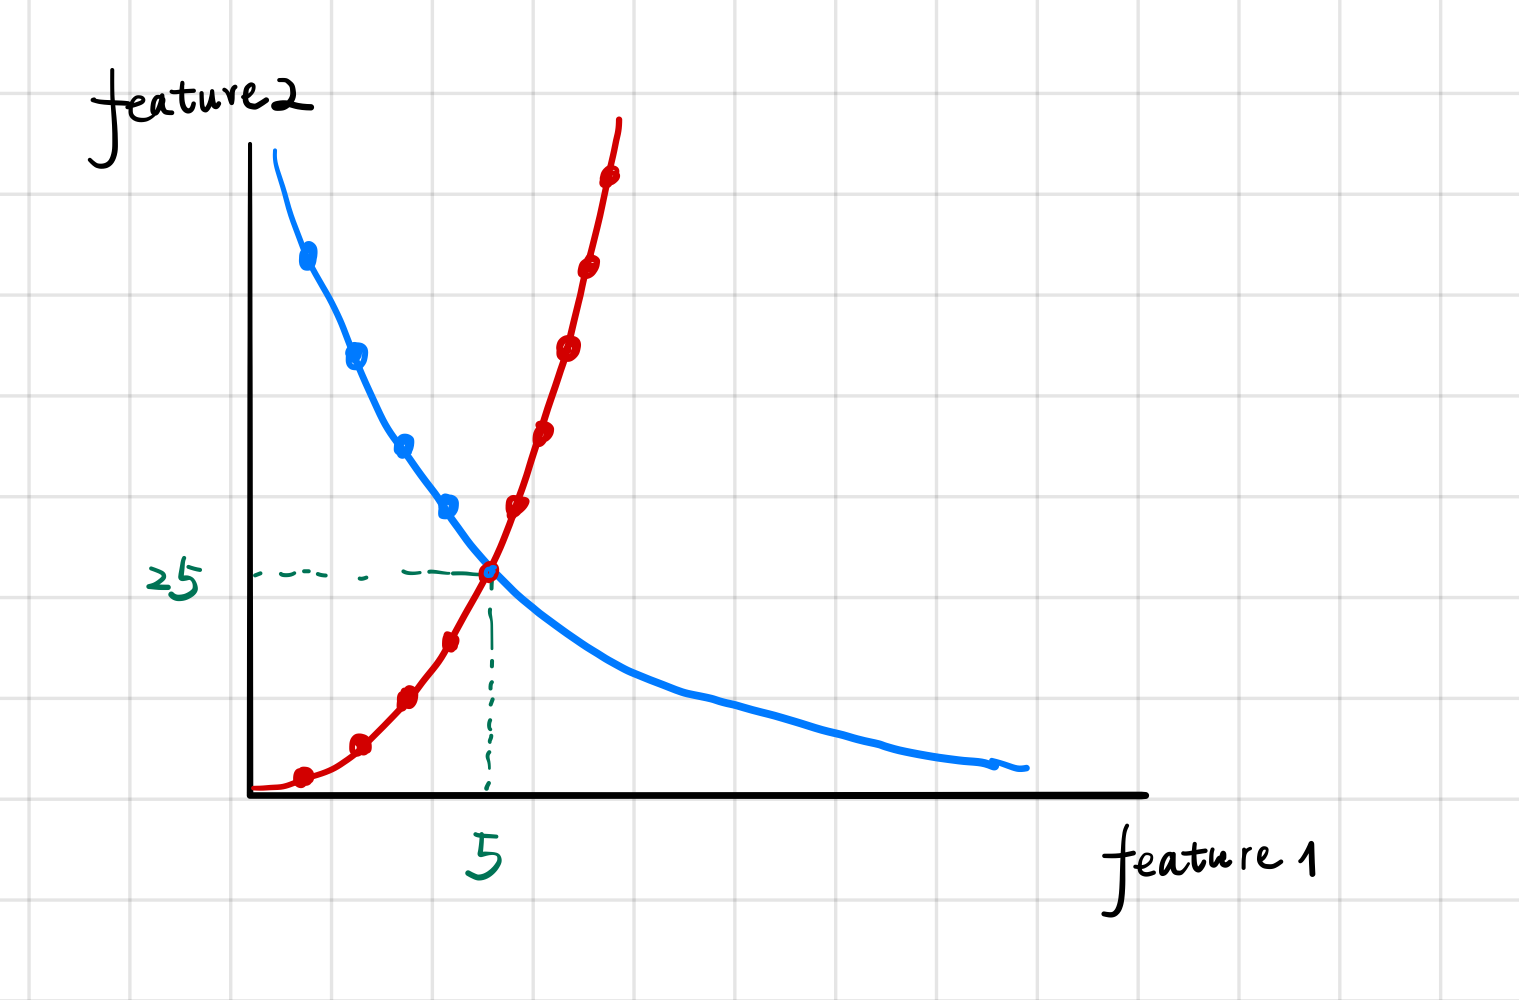
\includegraphics[width=0.7\textwidth]{Problem8.png} %插入图片,[]中设置图片大小,{}中是图片文件名
    \caption{the 2-d space of the dataset} %最终文档中希望显示的图片标题
    \label{Fig.main2} %用于文内引用的标签
  \end{figure}
  
  We can easily split the dateset into 4 parts.
  The first split uses the threshold \(\text{feaure2} \leqslant 25\). \\
  The second split uses the threshold \(\text{feature1} \leqslant 5\) for both child nodes. \\
  In this way, the depth of the decision tree is 2. Only one datapoint (5, 25) is missclassified,
  which is unavoidable.
\end{document}